\documentclass[compress]{beamer}

\mode<presentation>
{
\useoutertheme[subsection=false,footline=authorinstitutetitle]{miniframes}
\useinnertheme{rectangles}
\usecolortheme{whale}
\usecolortheme{orchid}
\usefonttheme{professionalfonts}

\setbeamertemplate{footline}
{
	\begin{beamercolorbox}[wd=0.33\textwidth,ht=2.2ex,dp=0.8ex,leftskip=1.4em,rightskip=1.4em]{author in head/foot}% 
		\usebeamerfont{author in head/foot}%
		\insertshortauthor%
	\end{beamercolorbox}%
 	\vspace*{-3.0ex}\hspace*{0.33\textwidth}%
 	\begin{beamercolorbox}[wd=0.33\textwidth,ht=2.2ex,dp=0.8ex,left,leftskip=1.4em,rightskip=1.4em]{author in head/foot}% 
     	\usebeamerfont{institute in head/foot}%
 		\insertshortinstitute%
 	\end{beamercolorbox}%
  	\begin{beamercolorbox}[wd=0.34\textwidth,ht=2.2ex,dp=0.8ex,left,leftskip=1.4em,rightskip=1.4em]{title in head/foot}
      	\usebeamerfont{title in head/foot}
  		\insertshorttitle
  		\hfill\insertframenumber\,/\,\inserttotalframenumber
  	\end{beamercolorbox}
}

\beamertemplatenavigationsymbolsempty
\setbeamercovered{transparent}

}


\usepackage[ngerman]{babel}
\usepackage[utf8]{inputenc}

% font definitions, try \usepackage{ae} instead of the following
% three lines if you don't like this look
\usepackage{mathpazo}
\usepackage[scaled=.90]{helvet}
%\usepackage{helvet}
\usepackage{courier}
\usepackage{graphics}
\usepackage{amsmath}
\usepackage{amsfonts}
\usepackage{amssymb}


\usepackage[T1]{fontenc}
\usepackage{multicol}
\usepackage{verbatim}
\usepackage{listings}
\usepackage{xcolor}

\newcommand{\textqt}[1]{\frqq #1\flqq\ }


\hypersetup{
   pdftitle={Verhaltensmuster: Observer, Command und Visitor},
   colorlinks=false,
   linkcolor=black,
   pdfpagemode=None,
   pdfstartview=Fit
  }

\author[Johannes Pfann]{%
  Johannes Pfann
}


\date{25.05.2016}

\institute[FAU Erlangen-Nürnberg]{
  Lehrstuhl für Software Engineering\\
  Friedrich-Alexander-Universität Erlangen-Nürnberg
}

\subject{Seminar Design Patterns und Anti-Patterns}
\title[Observer, Command, Visitor]{Verhaltensmuster\\Observer, Command, Visitor}

\newcommand{\changefont}[3]{
\fontfamily{#1}\fontseries{#2}\fontshape{#3}\selectfont}

\lstnewenvironment{beispiel}[3]{
    \lstset{language=#1, 
    numberbychapter=true,
    basicstyle=\ttfamily\small, 
    identifierstyle=\color{black}, 
    keywordstyle=\color{blue}, 
    stringstyle=\color{verde}, 
    commentstyle=\color{red}, 
   	breaklines=true, 
   	numbers=left,
   	label=#2,
   	caption=#3,
   	numberstyle=\small, 
   	frame=single}
   	\begingroup
   	\nopagebreak
   	}
   	{\endgroup}%  	   
   	

%%%%%% Farben 
\definecolor{hellgrau}{rgb}{0.95,0.95,0.95}
\definecolor{dunkelgrau}{rgb}{0.8,0.8,0.8}
\definecolor{dunkelgruen}{rgb}{69,139,0}
%\AtBeginSection[]
%{
%  \begin{frame}
%    \frametitle{Gliederung}
%    \tableofcontents[currentsection, hideothersubsections]
%  \end{frame}
%}

\AtBeginSection[]
{
  \begin{frame}
    \frametitle{Gliederung}
    \tableofcontents[currentsection, hideallsubsections]
  \end{frame}
}

\definecolor{dkgreen}{rgb}{0,0.6,0}
\definecolor{gray}{rgb}{0.5,0.5,0.5}
\definecolor{mauve}{rgb}{0.58,0,0.82}

\usepackage[section]{minted}
\definecolor{mintedbackground}{rgb}{0.95,0.95,0.95}

\newmintedfile[javacode]{java}{
	bgcolor=mintedbackground,
	linenos=true,
	numberblanklines=true,
	numbersep=5pt,
	gobble=0,
	funcnamehighlighting=true,
	tabsize=4,
	obeytabs=false,
	mathescape=false
	samepage=true,
	showspaces=false,
	showtabs =false,
	texcl=false,
	breaklines=true,
	fontsize=\scriptsize,
	style=trac
}


\begin{document}


\frame{\titlepage} 

\begin{frame}
	\frametitle{Gliederung}
	\tableofcontents[hideallsubsections]
\end{frame}


\section[Verhaltensmuster]{Verhaltensmuster}
\subsection*{Erzeugungsmuster - Was ist das?}
\begin{frame}
	\frametitle{Verhaltensmuster -- Was ist das?}
	\begin{block}{Verhaltensmuster ...}
	\begin{itemize}
		\item Zuweisung von Zuständigkeiten
		\item Wechselseitige Kommunikation zwischen Objekten
		\item Beschreibung von komplexen Programmabläufen
	\end{itemize}
	\end{block}	
	\begin{block}{Konsequenzen}
	\begin{itemize}
		\item Trennung von Verantwortlichkeiten
		\item Veringerung der Kopplung 
		\item Erhöhung der Flexibilität der Software hinsichtlich ihres Verhaltens
		\item Bessere Verständlichkeit eines Programmablaufes
	\end{itemize}
	\end{block}	
\end{frame}

\subsection*{Typen von Erzeugungsmustern}
\begin{frame}
	\frametitle{Typen von Erzeugungsmustern}
	\begin{block}{Klassenbasiert}
		Klassenbasierte Verhaltensmuster wenden für die VErhaltenszuordnung zu den Klassen das Vererbungsprinzip an. 
		\begin{itemize}
			\item Template Method
			\item Interpreter
		\end{itemize} 	
	\end{block}

	
\end{frame}

\begin{frame}
	\frametitle{Typen von Erzeugungsmustern}
	\begin{block}{Objektbasiert}
		Bei objektbasierten Mustern wird der Erzeugungsprozess an andere Objekte delegiert
				\begin{itemize}
					\item \alert<1-> {Observer}
					\item \alert<1-> {Command}
					\item \alert<1-> {Visitor}
					\item Strategy			
					\item Mediator
					\item Iterator
					\item Memento 
					\item State
					\item Chain of Responsibility
				\end{itemize}	
	\end{block}
\end{frame}


\section[Observer]{Observer}
\subsection{Definition}
\begin{frame}
  \frametitle{Definition}

  \begin{block}{Zweck}
  	Definition einer 1-zu-n-Abhängigkeit zwischen Objekten, damit im Fall einer Zustandsänderung eines Ojbekts alle davon abhängigen Objekte entsprechend benachrichtigt und automatisch aktualisiert werden.
  \end{block}
  	
  \begin{block}{Motivation/Ziel}
  	\begin{itemize}
  		\item asdf
  		\item asdf
  	\end{itemize}
  \end{block}
\end{frame}

\subsection{Klassendiagramm - Observer Pattern}
\begin{frame}
	\frametitle{Observer Pattern}
	\begin{itemize}
		\item Basiert auf Rollen
		\item Stellt Mechanismus zur Broadcast-Kommunikation dar
	\end{itemize}	
	
  	\begin{figure}
		\includegraphics[scale=.4]{paper/observer/observer}
	\end{figure}
\end{frame}


\subsection{Beispiel - Arbeitsvermittlung}
\begin{frame}
	\frametitle{Arbeitsvermittlung}
	\begin{itemize}
		\item 1-zu-n-Kommunikation zwischen Vermittlung und Klienten (Broadcast)
		\item Arbeitsvermittlung kennt weder Anzahl noch konkrete Klienten
		\item Klienten melden sich nur an, wenn sie daran interessiert sind.
	\end{itemize}		 
  	\begin{figure}
		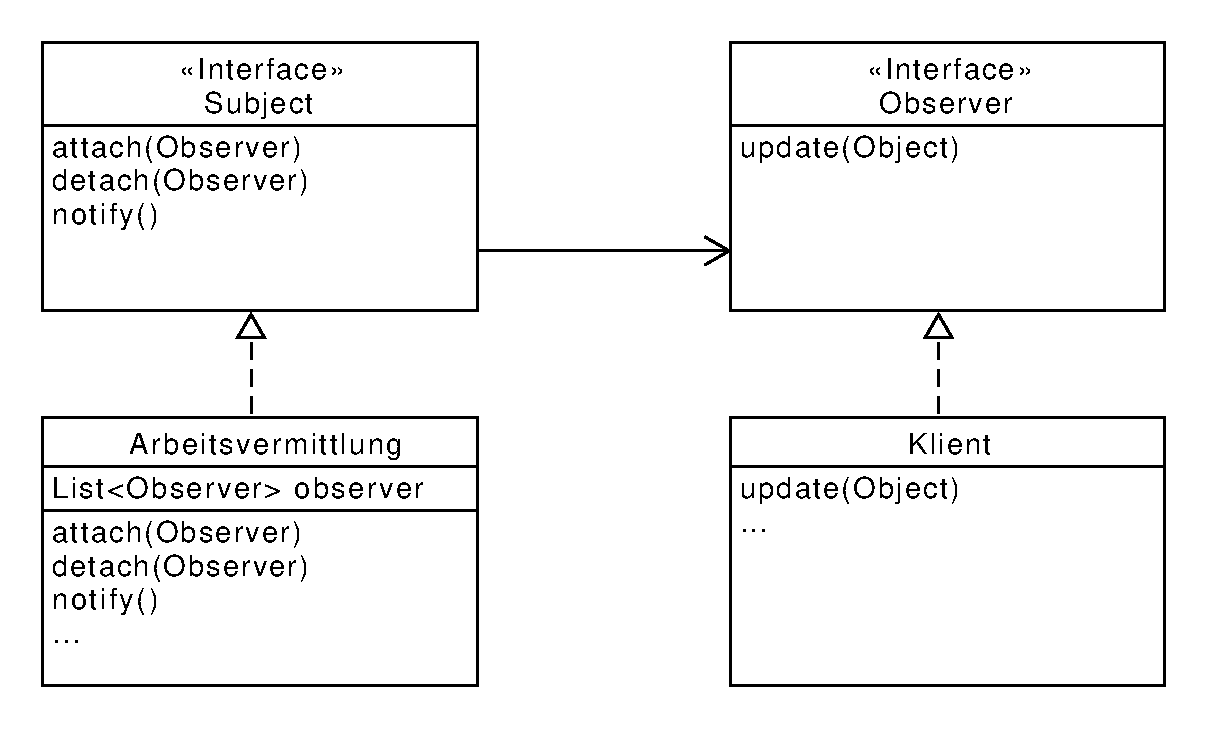
\includegraphics[scale=.4]{paper/observer/arbeitsvermittlung}
	\end{figure}
\end{frame}


\begin{frame}
\frametitle{Beispiel - Klient}
		\javacode{resources/observer_Subject_Interface.java} 
  		\javacode{resources/observer_Klient.java}	  
\end{frame}

\begin{frame}
\frametitle{Beispiel - Arbeitsvermittlung}
		\javacode{resources/observer_Observer_Interface.java}
  		\javacode{resources/observer_Arbeitsvermittlung.java}	  
\end{frame}

\subsection{Implementierungsmöglichkeiten}
\begin{frame}
\frametitle{Implementierungsmöglichkeiten}
		\begin{block}{Push Modell}
		  \begin{itemize}
		  	\item Daten nur in der update-Methode
		  	\item Zugriff auf Subject nicht erlaubt
		  	\item Subjekt muss Interesse der Observer kennen.
		  \end{itemize}
  		\end{block}
  		\begin{block}{Pull Modell}
  		 \begin{itemize}
		  	\item update-Methode ohne Parameter
		  	\item Zugriff auf Subjekt erwünscht
		  	\item Observer müssen Subject kennen
		  \end{itemize}  
  		\end{block}
  		Beides kann auch gemischt weden!
\end{frame}


\begin{frame}
\frametitle{Implementierungsmöglichkeiten}
		  \begin{block}{Observer beobachten mehrere Subects}
		  	\begin{itemize}
		  		\item Observer registriert sich bei mehreren Subjects
		  		\item Muss allerdings unterschiedlich darauf reagieren
		  		\item Lösung: erweiterung der update-Methode mit Subject
		  	\end{itemize}
		  \end{block}
		\javacode{resources/observer_erweiterung_update.java}  		
\end{frame}

\begin{frame}
\frametitle{Implementierungsmöglichkeiten}
		\begin{block}{Ausführung der Updates durch Subject}
  		 \begin{itemize}
		  	\item Weniger fehleranfällig
		  	\item Jedoch zu häufige Updates
		  \end{itemize}  
  		\end{block}		
  		\begin{block}{Ausführung der Updates durch Client}
		  \begin{itemize}
		  	\item Fehleranfälliger
		  	\item Regulierung der Updates
		  \end{itemize}
  		\end{block}
			
\end{frame}


\section[Command]{Command}
\subsection{Definition}
\begin{frame}
  \frametitle{Definition}
  \begin{block}{Zweck}
  	Kapselung eines Requests als Objekt, um so die Parametrisierung von Clients mit verschiedenen Requests, Warteschlangen- oder Logging-Operationen sowie das Rückgängigmachen von Operationen zu ermöglichen
  \end{block}
  
\end{frame}

\subsection{Klassendiagramm - Command Pattern}
\begin{frame}
	\frametitle{Observer Pattern}		
	\begin{itemize}
		\item Kapselt Request in ein eigenes Objekt Command
		\item Implementierung von Command kennt dann auch den Empfänger
	\end{itemize}	
  	\begin{figure}
		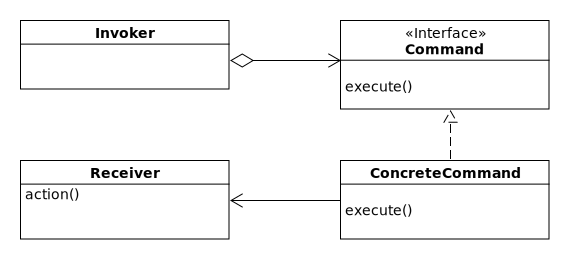
\includegraphics[scale=.4]{paper/command/command}
	\end{figure}
\end{frame}

\subsection{Beispiel - Deliver Service}
\begin{frame}
	\frametitle{Klassendiagramm}
	\begin{itemize}
		\item Verschiedene Objekte die unterschiedlich ausgeliefert werden müssen
		\item Unterschiedliche Kunden
	\end{itemize}	
	
  	\begin{figure}
		\includegraphics[scale=.4]{paper/command/DeliverService}
	\end{figure}
\end{frame}


\begin{frame}
	\frametitle{Command}
  	\begin{figure}
		\javacode{resources/command_interface.java} 
		\javacode{resources/command_DeliverBigPackageCommand.java} 
	\end{figure}
\end{frame}

\begin{frame}
	\frametitle{Command Interface}
  	\begin{figure}
		\javacode{resources/command_DeliveryService.java} 
		\javacode{resources/command_main.java}
	\end{figure}
\end{frame}

\subsection{Implementierung}

\begin{frame}
	\frametitle{Erweiterung}
  	\begin{block}{Undo-Funktion}
\begin{itemize}
		\item Erweiterung des Interfaces Command mit undo-Methode
		\item Der Invoker kann sich Commands merken und auf diese eine undo-Methode aufrufen
		\item das ConcreteCommand muss dann ggf. Daten speichern:
			\begin{itemize}
				\item Receiver-Objekt
				\item Die Argumente, die für die Ausführung angewendet wurden
				\item Alle relevanten Orginalwerte im Receiver-Objekt
			\end{itemize}
	\end{itemize}	
   \end{block}
\end{frame}

\begin{frame}
	\frametitle{Erweiterung}
  	\begin{block}{Makro-Befehle}
		\begin{itemize}
			\item Mehrere Receiver könnten gleichzeitig durch ein Command bearbeitet werden
		\end{itemize}	
   \end{block}
   \javacode{resources/command_macro_command.java}
\end{frame}



\begin{frame}
	\frametitle{Implementierungsmöglichkeit}
  	\begin{block}{Intelligenz der Commandobjekte}
		\begin{itemize}
		\item Command übernimmt vollständig die Logik
		\item Comnand delegiert die komplette Logik an den Receiver
	\end{itemize}	
   \end{block}
   
		\javacode{resources/command_command_logic.java}
		\javacode{resources/command_command_logic.java}
  
\end{frame}


\subsection{Fazit}
\begin{frame}
	\frametitle{Fazit}
	\begin{columns} 
    	\column[t]{.50\textwidth} 
    		\begin{exampleblock}{Vorteile}
    			\begin{itemize}
    				\item Entkopplung von Befehl und Ausführung
    				\item Aufrufer können mit dem Interface Command arbeiten ohne wissen zu müssen, welche Operationen hinter den konkreten Commands stecken
    				\item Flexiblität indem Commands leicht ausgetauscht werden können
    			\end{itemize}
    		\end{exampleblock}
    	\column[t]{.50\textwidth} 
    		\begin{alertblock}{Nachteile}
    			\begin{itemize}
    				\item Hohe Anzahl von Klassen
    			\end{itemize}
    		\end{alertblock}
  	\end{columns}   	  		
\end{frame}

\section[Visitor]{Visitor}
\subsection{Definition}
\begin{frame}
  \frametitle{Definition}
  \begin{block}{Zweck}
Das Visitor Pattern ermöglicht es, neue Operationen auf den Elementen einer Struktur zu definieren, ohne die Elemente selbst anzupassen.
  \end{block}
\end{frame}

\subsection{Klassendiagramm - Visitor Pattern}
\begin{frame}
	\frametitle{Klassendiagramm}		
	\begin{itemize}
		\item Anzahl unterschiedlicher Elemente der Objektstruktur fest
	\end{itemize}	
  	\begin{figure}
		\includegraphics[scale=.3]{paper/visitor/visitor}
	\end{figure}
\end{frame}

\subsection{Beispiel - Kitchen}
\begin{frame}
	\frametitle{Beispiel}
	\begin{itemize}
		\item Die verschiedenen Sorten die wir bearbeiten möchten, bleiben konstant
		\item Wie wir diese bearbeiten ist noch unklar.
	\end{itemize}	
	
  	\begin{figure}
		\includegraphics[scale=.3]{paper/visitor/kitchen}
	\end{figure}
\end{frame}



\begin{frame}
	\frametitle{Beispiel}
  	\begin{figure}
		\javacode{resources/visitor_element_interface.java} 
		\javacode{resources/visitor_visitor_interface.java}
	\end{figure}
\end{frame}

\begin{frame}
	\frametitle{Beispiel}
  	\begin{figure}
		\javacode{resources/visitor_potato.java} 
		\javacode{resources/visitor_cleanvisitor.java}
	\end{figure}
\end{frame}

\begin{frame}
	\frametitle{Beispiel}
  	\begin{figure}
		\javacode{resources/visitor_main.java} 
	\end{figure}
\end{frame}

\begin{frame}
	\frametitle{Beispiel}		
	\begin{itemize}
		\item Der Client erstellt die Instanzen cleanVisitor, potato und broccoli
		\item Übergibt Elemente über Accept-Methode(potato und broccoli) den Visitor
		\item Elemente rufen die jeweilige Visit-Methode auf und übergeben sich selbst
		\item Der Visitor bearbeitet dann das übergebene Element
	\end{itemize}	
  	\begin{figure}
		\includegraphics[scale=.6]{paper/visitor/visitor_sequenz}
		                                        
	\end{figure}
\end{frame}




\begin{frame}
	\frametitle{Implementierungsmöglichkeiten}
  \begin{block}{Wer ist für die Traversierung der Objektstruktur verantwortlich}
  	\begin{itemize}
  		\item Die Objektstuktur
  		\item Ein Iterator
  		\item Das Visitor-Objekt
  	\end{itemize}
  \end{block}
\end{frame}


\begin{frame}
	\frametitle{Implementierungsmöglichkeiten}
  \begin{block}{Objektstruktur}
  	\begin{itemize}
  		\item Objektstruktur kümmert sich um die Traversierung 
  		\item Visitor muss der Objektstruktur übergeben werden
  		\item Realisierbar durch z.B Composide-Pattern
  	\end{itemize}
  \end{block}
  \javacode{resources/visitor_composide_example.java} 
\end{frame}

\begin{frame}
	\frametitle{Implementierungsmöglichkeiten}
  \begin{block}{Iterator}
  	\begin{itemize}
  		\item Abstraktion zum Zugriff auf Elemente einer Objektstruktur, ohne die  Objektstruktur zu kennen.
  		\item Visitor-Objekt wird dem Iterator übergeben
  		\item Beim Zugriff eines Elements die accept-Methode aufrufen

  	\end{itemize}
  \end{block}
	\begin{block}{Im Visitor-Objekt}
  	\begin{itemize}
  		\item Objektstruktur wird den konkreten Visitors übergeben
  		\item Visitor übernimmt jetzt die Traversierung
  		\item Nachteil: Traversierung in jedem Visitor
  		\item Vorteil: Möglichkeit, die Objektstruktur unterschiedlich zu durchlaufen
  	\end{itemize}
  \end{block}
\end{frame}


\begin{frame}
	\frametitle{Implementierungsmöglichkeiten}

  \javacode{resources/visitor_trav_visitor_object.java} 
\end{frame}

\subsection{Fazit}
\begin{frame}
	\frametitle{Fazit}
	\begin{columns} 
    	\column[t]{.50\textwidth} 
    		\begin{exampleblock}{Vorteile}
    			\begin{itemize}
    				\item Leicht neue Operationen auf eine Objektstruktur zu implementieren
    				\item Selektives bearbeiten einzelner Elemente einer Objektstruktur
    			\end{itemize}
    		\end{exampleblock}
    	\column[t]{.50\textwidth} 
    		\begin{alertblock}{Nachteile}
    			\begin{itemize}
    				\item Enge Kopplung des Visitor mit den Elementen einer Objektstruktur
    				\item Elemente müssen über öffentliche Methoden und Attribute den Zugriff bereitstellen
    			\end{itemize}
    		\end{alertblock}
  	\end{columns}   	  		
\end{frame}

\section{Zusammenfassung}
\begin{frame}
  \frametitle{Zusammenfassung}
  \begin{block}{Observer}
	\begin{itemize}
		\item 1-zu-n-Abhängikgeit
		\item Subjects benachrichtigen Observer bei Zustandsänderung
	\end{itemize}
  \end{block}
  \begin{block}{Command}
	 \begin{itemize}
		\item Kapselung eines Requests als Objekt
		\item Invoker kann flexibel Requests austauschen
	 \end{itemize}
   \end{block}
  \begin{block}{Visitor}
	 \begin{itemize}
		\item Definition neuer Operationen auf Elemente einer Struktur
		\item Elemente müssen nicht angepasst werden
	 \end{itemize}
    \end{block}
\end{frame}


\section[Quellen]{Quellen}
\begin{thebibliography}{5cm}
 \bibitem[1]{1} Gamma, Helm, Johnson, Vlissides: „Design Patterns -
Entwurfsmuster als Elemente wiederverwendbarer
Objektorientierter Software“.
1. Auflage, mitp Verlags GmbH, 2015.
   \bibitem[2]{2} Eilebrecht, Starke: „Patterns Kompakt - Entwurfsmuster für
effektive Software-Entwicklung“.
3. Auflage, Spektrum Verlag, Heidelberg 2010.
   \bibitem[3]{3} Michael Inden: Der Weg zum Java-Profi. 3 Auflage dpunkt.verlag
 \bibitem[4]{4} Eric Freeman, Elisabeth Freeman, Kathy Sierra, Bert Bates: Entwurfsmuster von Kopf bis Fuß. 1 Auflage O'Reilly Media, Inc
\end{thebibliography}



\end{document}

